% This must be in the first 5 lines to tell arXiv to use pdfLaTeX, which is strongly recommended. \pdfoutput=1
% In particular, the hyperref package requires pdfLaTeX in order to break URLs across lines.

\documentclass[11pt]{article}

% Remove the "review" option to generate the final version.
\usepackage{ACL2023}

% Standard package includes
\usepackage{times}
\usepackage{latexsym}
\usepackage{graphicx} % Add the graphicx package for including images

% For proper rendering and hyphenation of words containing Latin characters (including in bib files)
\usepackage[T1]{fontenc}
% For Vietnamese characters
% \usepackage[T5]{fontenc}
% See https://www.latex-project.org/help/documentation/encguide.pdf for other character sets

% This assumes your files are encoded as UTF8
\usepackage[utf8]{inputenc}

% This is not strictly necessary, and may be commented out.
% However, it will improve the layout of the manuscript,
% and will typically save some space.
\usepackage{microtype}

% This is also not strictly necessary, and may be commented out.
% However, it will improve the aesthetics of text in
% the typewriter font.
\usepackage{inconsolata}

\newcommand{\customsection}[1]{
  \noindent\textbf{#1}.\vspace{2mm}
}

% If the title and author information does not fit in the area allocated, uncomment the following
%
%\setlength\titlebox{<dim>}
%
% and set <dim> to something 5cm or larger.

\title{Instructions for ACL 2023 Proceedings}

\author{Martínez, Camilo \\
  Universität des Saarlandes \\
  \texttt{cama00005@uni-saarland.de} \\\And
  Ma, Honglu \\
  Universität des Saarlandes \\
  \texttt{homa00001@uni-saarland.de} \\}

\begin{document}
\maketitle
\begin{abstract}
    This paper presents a comprehensive evaluation of multilingual representation spaces using pre-trained models, conducted as part of the Neural Networks: Theory and Implementation at Universität des Saarlandes. We examine the hidden representations of language models across various languages. Our study focuses on a subset of six languages and employs dimensionality reduction techniques, PCA and t-SNE, to visualize and interpret high-dimensional spaces on the context of language embeddings. We acknowledge the limitations posed by computational resources, which restrict batch sizes and the number of languages analyzed. We fine-tuned the model xglm-564M on a Quechua dataset and compared the performance of the original model with the fine-tuned versions. We also implemented and compared the performance of different fine-tuning methods, including full fine-tuning, BitFit, LoRA, and (IA)\textsuperscript{3}.
\end{abstract}

% \section{Introduction}

% These instructions.

% \section{Background}

% hola

\section{Experiments and Results}

\subsection{Dimensionality Reduction Techniques}

For PCA visualizations, we used the standard PCA implementation from the scikit-learn library. We used the default parameters for the PCA algorithm, recommended by the library's documentation. Unlike t-SNE, PCA does not need to be fine-tuned, as it is a deterministic algorithm.

On the other hand, for the t-SNE visualizations, we used the parameters recommended on various papers such as \cite{GOVE202287}, \cite{Weber2023}, where they recommended to try out perplexities on the range of [1, 50], focusing on bigger numbers for big datasets. ALso, for the learning-rate of the algorithm, they recommend to take $\max{(200, n / 12)}$ as an appropriate value, where $n$ is the number of samples in the dataset.

\subsection{Fine-tuning the XGLM-564M Model}
\customsection{Full-finetuning} We implemented a full finetuning approach, where the entire model's weights are relearned on the target task from scratch.
A full fine tuning on a pretrained model is a common practice in NLP. It is a simple and effective way to adapt a model to a specific task.
To do a full fine tune, we first need to supply the existing model new data to train from.
As its name suggested, a full fine tuning can be very time consuming and computationally expensive
As the model is traning every parameters again specifically for the new task, it is also more prone to overfitting.

We started Task 3 by finding a Quechua dataset on HuggingFace
where we found a dataset with pure Quechua sentences.
After the fine tuning, our model gained a significant drop in loss (5.5) with only 8192 data points.
(The original dataset has 80k data points which is too big for our machine to handle)

Although the loss is lower than the previous pretrained model,
it takes a long time to train with the reason specified above.

\customsection{BitFit} We implemented Simple Parameter efficient Fine-tuning
for Transformer-based Masked Language-models, BitFit \cite{zaken2022bitfit}.
BitFit is a simple method to fine tune a model. 
Since it only performs gradient decent on bias term, it is much faster than full fine tuning.
However, it is also result in a less accurate model with a higher loss.

\customsection{LoRA} We implemented a Low-Rank Adaptation of Large Language Models or LoRA, introduced in the paper \cite{hu2021lora}.
Instead of training the whole matrix which has a size of $nxm$, LoRA only trains two smaller matrices with a size of $nxr$ and $mxr$
where $r$ is the smaller than the rank of the original matrix.
This results in a smaller number of trainable parameters and thus, a faster training time.
Our model's training result corresponds to the paper's result.
Since LoRA approximates the weight matrix, it still has a higher loss than the full fine tuning method but 
a better result than BitFit.
The training time is similar but slightly more than BitFit which is also caused by number of trainable parameters as expected.

\customsection{} We implemented a PEFT method called (IA)\textsuperscript{3} that scales activations by learned vectors, attaining stronger performance while only introducing a relatively tiny amount of new parameters, as introduced in the paper \cite{liu2022fewshot}.
(IA)\textsuperscript{3} is a method very similar to LoRA. Instead of training two smaller matrices to approximate the original one,
it trains a vector to scale the activations of the model, i.e. a vector being multiplied to the output of activation function.
Since an element-wise multiplication is also some sort of matrix transformation, it is an analog to LoRA.
For each layer, IA3 trains three vectors which corresponds to scale the result of the key projection, the value projection and the activation function.
Unfortuneately, due to a lack of computational resource and time, our IA3 model is not showing promising result.
As the paper stated, we embeded three trainable vectors to each layer.

\subsection{Plots}

Some of the visualizations of the hidden representations of the sentences and tokens for the XGLM-564M model are shown in the Appendix.

The model performance plots were as follows (the rest of the plots are in: \url{https://wandb.ai/hwga-cj/xglm-full})

\begin{figure}[h]
    \centering
    \includegraphics[width=0.5\textwidth]{plots/xglm_vs_gpt2_mean_losses.png}
    \caption{Loss of the XGLM-564M Model compared to GPT-2}
\end{figure}

\begin{figure}[h]
    \centering
    \includegraphics[width=0.5\textwidth]{plots/xglm_vs_finetuned.png}
    \caption{Loss of XGLM-564M Model compared to its fine-tuned versions}
\end{figure}

\section{Conclusions}


\section*{Limitations}
Due to the extensive computational requirements, the study was limited to a batch size of 2. This constraint could potentially affect the generalization of the findings. For instance, larger batch sizes may yield different embeddings and therefore, the representations of the hidden-layers of the model and potentially alter the provided PCA and t-SNE visualizations. Additionally, the analyses were focused on a selection of six languages: English, Spanish, German, Arabic, Tamil, and Quechua. Therefore, the results presented may not be universally applicable, particularly to languages with much different structures.

Furthermore, for the sensible feasibility of t-SNE computations on our datasets, we employed the fast implementation provided via the openTSNE library \cite{opentsne}, given our computational resources constraints. Although our study utilized the CS cluster, the requirement for substantial GPU resources limits the scalability of our methods, particularly for longer texts or larger datasets. This presents an avenue for further research to develop more resource-efficient algorithms capable of handling more extensive and linguistically diverse data without compromising on the fidelity of the representations.

\section*{Ethics Statement}
Our review work strictly adheres to the ACL Ethics Policy.\footnote{\url{https://www.aclweb.org/portal/content/acl-code-ethics}} We acknowledge that while our evaluation contributes to the understanding of language model behaviors and their applications, it does not introduce novel methodologies or data. We have carefully considered the ethical implications of our work, ensuring that our analyses do not misrepresent capabilities, and we recognize the importance of responsible AI development and the potential impact of language technologies on society. Our work aims to provide a comprehensive, unbiased evaluation to foster informed discussions within the research community. This review has been conducted with an emphasis on transparency and reproducibility, encouraging the ethical advancement of natural language processing research.

\section*{Acknowledgements}
This work was conducted as a final project for the course "Neural Networks: Theory and Implementation," instructed by Prof. Dietrich Klakow at Universität des Saarlandes. We extend our gratitude to the course's Team for their guidance on this project and to the University. This document format and styling has been adapted by Jordan Boyd-Graber, Naoaki Okazaki, Anna Rogers from the style files used for earlier ACL, EMNLP and NAACL proceedings, including those for
EACL 2023 by Isabelle Augenstein and Andreas Vlachos,
EMNLP 2022 by Yue Zhang, Ryan Cotterell and Lea Frermann,
ACL 2020 by Steven Bethard, Ryan Cotterell and Rui Yan,
ACL 2019 by Douwe Kiela and Ivan Vuli\'{c},
NAACL 2019 by Stephanie Lukin and Alla Roskovskaya,
ACL 2018 by Shay Cohen, Kevin Gimpel, and Wei Lu,
NAACL 2018 by Margaret Mitchell and Stephanie Lukin,
Bib\TeX{} suggestions for (NA)ACL 2017/2018 from Jason Eisner,
ACL 2017 by Dan Gildea and Min-Yen Kan, NAACL 2017 by Margaret Mitchell,
ACL 2012 by Maggie Li and Michael White,
ACL 2010 by Jing-Shin Chang and Philipp Koehn,
ACL 2008 by Johanna D. Moore, Simone Teufel, James Allan, and Sadaoki Furui,
ACL 2005 by Hwee Tou Ng and Kemal Oflazer,
ACL 2002 by Eugene Charniak and Dekang Lin,
and earlier ACL and EACL formats written by several people, including
John Chen, Henry S. Thompson and Donald Walker.
Additional elements were taken from the formatting instructions of the \emph{International Joint Conference on Artificial Intelligence} and the \emph{Conference on Computer Vision and Pattern Recognition}.

% Entries for the entire Anthology, followed by custom entries
\bibliography{anthology,custom}
\bibliographystyle{acl_natbib}

\appendix

\section{Appendix: Plots}
\label{sec:appendix}

\begin{figure}[h]
    \centering
    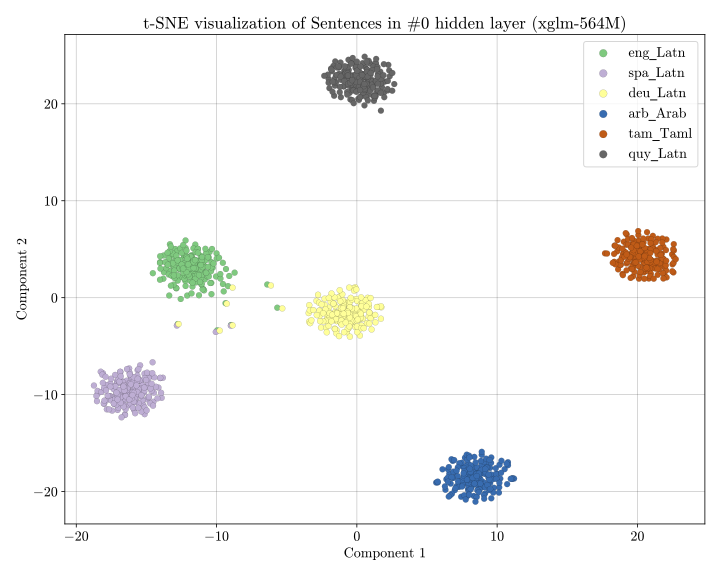
\includegraphics[width=0.5\textwidth]{plots/sentence_xglm-564M_layer_0_t-SNE.png}
    \caption{t-SNE Visualization of Hidden Representations of Sentences for Layer 0 of the XGLM-564M Model}
\end{figure}

\begin{figure}[h]
    \centering
    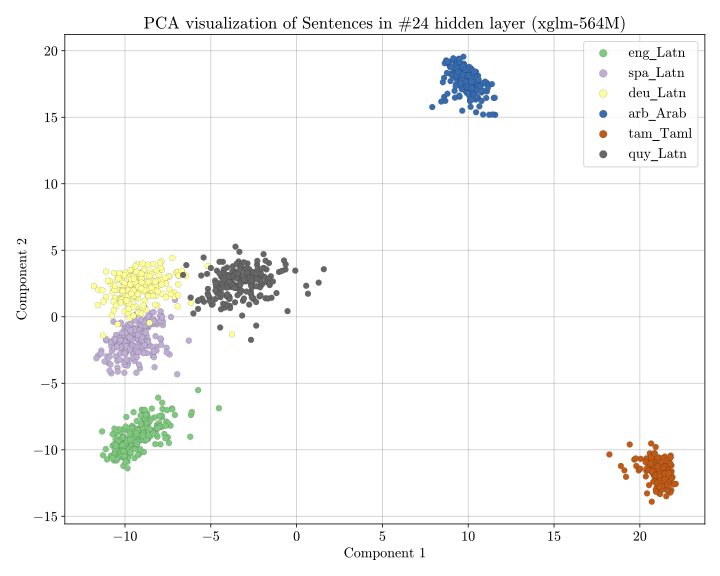
\includegraphics[width=0.5\textwidth]{plots/sentence_xglm-564M_layer_24_PCA.png}
    \caption{PCA Visualization of Hidden Representations of Sentences for Layer 24 of the XGLM-564M Model}
\end{figure}
\begin{figure}[h]
    \centering
    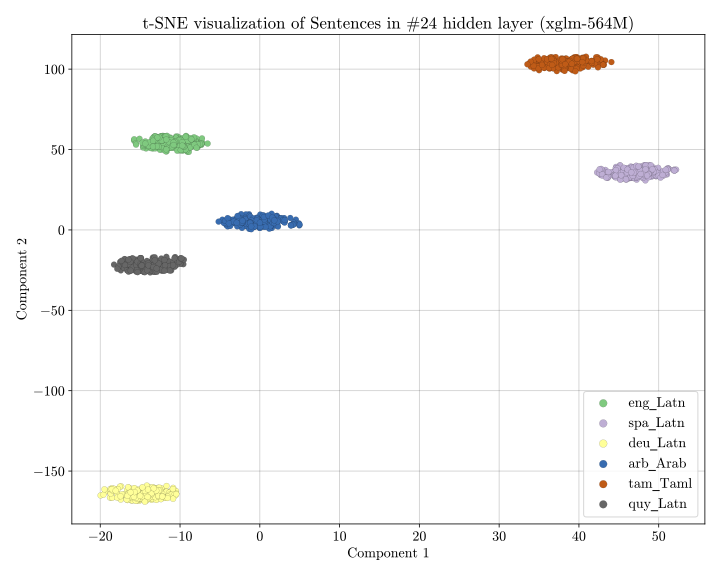
\includegraphics[width=0.5\textwidth]{plots/sentence_xglm-564M_layer_24_t-SNE.png}
    \caption{t-SNE Visualization of Hidden Representations of Sentences for Layer 24 of the XGLM-564M Model}
\end{figure}

\begin{figure}[h]
    \centering
    \includegraphics[width=0.5\textwidth]{plots/token_xglm-564M_layer_0_PCA.png}
    \caption{PCA Visualization of Hidden Representations of Tokens for Layer 0 of the XGLM-564M Model}
\end{figure}

\begin{figure}[h]
    \centering
    \includegraphics[width=0.5\textwidth]{plots/token_xglm-564M_layer_0_t-SNE.png}
    \caption{t-SNE Visualization of Hidden Representations of Tokens for Layer 0 of the XGLM-564M Model}
\end{figure}

\begin{figure}[h]
    \centering
    \includegraphics[width=0.5\textwidth]{plots/token_xglm-564M_layer_24_PCA.png}
    \caption{PCA Visualization of Hidden Representations of Tokens for Layer 24 of the XGLM-564M Model}
\end{figure}

\begin{figure}[h]
    \centering
    \includegraphics[width=0.5\textwidth]{plots/token_xglm-564M_layer_24_t-SNE.png}
    \caption{t-SNE Visualization of Hidden Representations of Tokens for Layer 24 of the XGLM-564M Model}
\end{figure}


\end{document}

% Table~\ref{citation-guide} shows the syntax supported by the style files.
% We encourage you to use the natbib styles.
% You can use the command \verb|\citet| (cite in text) to get ``author (year)'' citations, like this citation to a paper by \citet{Gusfield:97}.
% You can use the command \verb|\citep| (cite in parentheses) to get ``(author, year)'' citations \citep{Gusfield:97}.
% You can use the command \verb|\citealp| (alternative cite without parentheses) to get ``author, year'' citations, which is useful for using citations within parentheses (e.g. \citealp{Gusfield:97}).